
\section{Implementation}

In this section we first present a micro benchmark to validate our investigation of entity approximation and compression.
We then discuss the implementation of the compression and approximation techniques over a large real-world
cross-document coreference corpus.

\subsection{Microbenchmark}
\label{sec:microbenchmark}
To increase our intuition of early stopping techniques we simulated the MCMC proposal processes. 
We hypothesis that there is a clear range values where performing the
baseline cluster sampling would be faster when compared to early stopping methods.
We arrange entity clusters of increasing time and we compute the time (in clock ticks)
each proposal takes to compute the arrangement of the clusters.
The data in the clusters are distributed uniformly and for this experiment each cluster point
was 5 dimensional.
For the baseline cluster score computation we used a pairwise calculated of the average cosine distance
with and without the mention.
To compute early stopping we set a confidence threshold to $0.8$ and the early
stopping code stopped computation when the error predation was under $20\%$.
There was no difference in the proposal choices between the baseline and the early sorting method. 

The simulations were developped in \texttt{GNU C++11} and compiled with \texttt{g++ -O3}. 
The CPU was an 8 core intel i7 with 3.2 HGz and 12 GBs of Memory.
Each arrangement was run 5 times and results averages.


Experiment Results\ldots
The result of this experiment is summarized in Figure~\ref{fig:clustering-v-early-stopping}.
On the x-axis is the number of mentions in the source and destination clusteris for each proposal. 
The y-axsis is the number of clock ticks on a log scale.

\begin{figure}
\centering
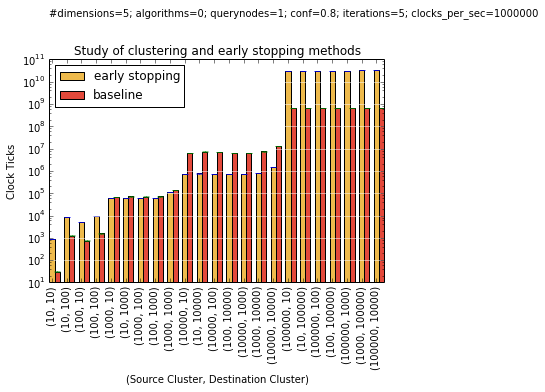
\includegraphics[width=\columnwidth, clip=true,trim=0cm 0cm 0cm 1.2cm]{media/clustering-v-early-stopping.png}
\caption{Comparison of baseline verses early stopping methods.}
\label{fig:clustering-v-early-stopping}
\end{figure}

We observe that for proposals with less than 100 and 1000 source and
destination mentions, the performance of the baseline proposer is better than
or almost equal to that of the more sorted early stopping method.
For proposals that contain an entity cluster with 10000 mentions
the early stopping method performs significantly better than the baseline method.

Surprisingly, the baseline proposals for for entities clusters containing $100 K$ mentions
performed over an order of magnitude better than the early stopping method.

The optimization found in predictable code paths make simple implementations
like the baseline method attractive for small cluster sizes and very large clusters sizes.
In addition, $82\%$ of the entities in the truthed Wiki-Links data sets are less
that 1000 mentions in size and $45\%$ of the entities contain less than 100
mentions.

The results of the microbenchmark suggests that different proposal estimation
techniques are useful at different times.



\subsection{Wiki Link Corpus}

The Wikilinks corpus is the largest fully labeled cross-document coreference resolution data set to date~\cite{singh12:wiki-links}.
When downloaded, the data set contains 40 million mentions and almost three million entities --- it is a compressed 180 GBs of data.
The wikilink corpus was created by crawling pages across the web and extracting anchor tags that referenced wikipedia articles.
Each page contains multiple multiple mentions of different types.
The wikipedia articles act as the truth for each mention.

